% Options for packages loaded elsewhere
\PassOptionsToPackage{unicode}{hyperref}
\PassOptionsToPackage{hyphens}{url}
%
\documentclass[
]{article}
\usepackage{lmodern}
\usepackage{amssymb,amsmath}
\usepackage{ifxetex,ifluatex}
\ifnum 0\ifxetex 1\fi\ifluatex 1\fi=0 % if pdftex
  \usepackage[T1]{fontenc}
  \usepackage[utf8]{inputenc}
  \usepackage{textcomp} % provide euro and other symbols
\else % if luatex or xetex
  \usepackage{unicode-math}
  \defaultfontfeatures{Scale=MatchLowercase}
  \defaultfontfeatures[\rmfamily]{Ligatures=TeX,Scale=1}
\fi
% Use upquote if available, for straight quotes in verbatim environments
\IfFileExists{upquote.sty}{\usepackage{upquote}}{}
\IfFileExists{microtype.sty}{% use microtype if available
  \usepackage[]{microtype}
  \UseMicrotypeSet[protrusion]{basicmath} % disable protrusion for tt fonts
}{}
\makeatletter
\@ifundefined{KOMAClassName}{% if non-KOMA class
  \IfFileExists{parskip.sty}{%
    \usepackage{parskip}
  }{% else
    \setlength{\parindent}{0pt}
    \setlength{\parskip}{6pt plus 2pt minus 1pt}}
}{% if KOMA class
  \KOMAoptions{parskip=half}}
\makeatother
\usepackage{xcolor}
\IfFileExists{xurl.sty}{\usepackage{xurl}}{} % add URL line breaks if available
\IfFileExists{bookmark.sty}{\usepackage{bookmark}}{\usepackage{hyperref}}
\hypersetup{
  pdftitle={A co-expression network analysis on European and American maize},
  hidelinks,
  pdfcreator={LaTeX via pandoc}}
\urlstyle{same} % disable monospaced font for URLs
\usepackage{longtable,booktabs}
% Correct order of tables after \paragraph or \subparagraph
\usepackage{etoolbox}
\makeatletter
\patchcmd\longtable{\par}{\if@noskipsec\mbox{}\fi\par}{}{}
\makeatother
%Set text alignment and size
\usepackage{subfig}
\usepackage{titling}
\pretitle{\begin{flushleft}\Huge\textbf}
\posttitle{\par\end{flushleft}}
\preauthor{\begin{flushleft}\large}
\postauthor{\end{flushleft}}
\predate{\begin{flushleft}}
\postdate{\end{flushleft}}
%Set caption alignment
\usepackage[singlelinecheck=false,justification=justified]{caption}
% Allow footnotes in longtable head/foot
\IfFileExists{footnotehyper.sty}{\usepackage{footnotehyper}}{\usepackage{footnote}}
\makesavenoteenv{longtable}
\usepackage{graphicx}
\usepackage{float}
\makeatletter
\def\maxwidth{\ifdim\Gin@nat@width>\linewidth\linewidth\else\Gin@nat@width\fi}
\def\maxheight{\ifdim\Gin@nat@height>\textheight\textheight\else\Gin@nat@height\fi}
\makeatother
% Scale images if necessary, so that they will not overflow the page
% margins by default, and it is still possible to overwrite the defaults
% using explicit options in \includegraphics[width, height, ...]{}
\usepackage[a4paper, top=20mm, bottom=25mm, left=15mm, right=15mm]{geometry}
\setkeys{Gin}{width=\maxwidth,height=\maxheight,keepaspectratio}
% Set default figure placement to htbp
\makeatletter
\def\fps@figure{htbp}
\makeatother
\setlength{\emergencystretch}{3em} % prevent overfull lines
\providecommand{\tightlist}{%
  \setlength{\itemsep}{0pt}\setlength{\parskip}{0pt}}
\setcounter{secnumdepth}{-\maxdimen} % remove section numbering

\title{\protect\hypertarget{_heading=h.monioe1wkcaf}{}{}\textbf{A co-expression network
analysis on European and American maize}}

% Author contains Author and supervisor
\author{\textbf{Author:} Jan Izquierdo i Ramos\\
	\textbf{Supervisor:} Dr. Georg Haberer}%Author end

% Date contains date and Institutions (samll+italics for institutions)
\date{March 2025\\ %date
\small \textit{Bachelor's Degree in Bioinformatics - UPF, UPC, UB, UAB\\ %Institutions
Plant Genome and Systems Biology - Helmholtz Munich}
}

\begin{document}
\maketitle

\hypertarget{introduction}{%
\section{Introduction}\label{introduction}}


Gene expression serves as a fundamental indicator of gene function, it
provides critical insights into the biological activity of an organism.
The transcription of a gene into RNA is a crucial step in gene activity,
therefore, it is highly regulated. This regulation is both temporal and
spatial, ensuring that genes are expressed in specific tissues at
concrete developmental stages and is essential for orchestrating complex
biological processes. Because of its importance this regulation has been
studied extensively, comprehensive gene expression atlases have been
established to capture these patterns in many model organisms.

This specificity of expression allows for the detection of the function
of a gene in a specific time and tissue. Beyond detection in
development, dynamic changes in gene expression serve as clues to
identify environmental stimuli or other external stressors because they
can serve as a response to these.

By the analysis of expression patterns, researchers can infer gene
functions, regulatory networks are discovered and better understandings
of organism adaptability are reached.

To analyze gene expression it has to be measured, there are several
techniques that can be used, early methods included qPCR and Northern
blots, which only allowed tracking of the expression of one gene,
nowadays RNA-seq is the preferred, and widely used, technique as it
allows for genome-wide expression profiling. RNA-seq bases the gene
expression in the number of sequencing reads that align to a given gene.
These are a direct measurement of transcript abundance and require
distinct statistics and methods to ensure compatibility in comparisons.
To account for differences in sequencing depth and gene length different
approaches exist:

\begin{itemize}
\item
  \begin{quote}
  Transcripts per million (TPM): Takes into account gene length and
  total sequencing depth, ensuring that expression values sum to one
  million across a sample.
  \end{quote}
\item
  \begin{quote}
  Counts per million (CPM): Adjusts for sequencing depth by scaling
  counts per million mapped reads.
  \end{quote}
\item
  \begin{quote}
  Reads per kilobase per million mapped reads (RPKM): Normalizes by
  both, individual gene length and sequencing depth.
  \end{quote}
\end{itemize}

The primary objective of normalization is to detect differentially
expressed genes (DEG), genes in which significant expression differences
can be observed between tissues, developmental stages or environmental
conditions. Traditional expression analyses are generally being phased
out because they focus on comparing the expression of individual genes,
however, genes rarely function in isolation, they rather operate within
a biological context, forming coordinated units named functional
modules. To map and understand these complex module relationships,
approaches that extend beyond single-gene analysis are used, gene
co-expression networks.

\hypertarget{gene-co-expression}{%
\subsection{Gene co-expression}\label{gene-co-expression}}

Gene co-expression refers to the coordinated expression of genes across
tissues, developmental stages or environmental conditions. The typical
co-expression analysis employs pairwise comparisons of gene expression
levels, identifying genes that show similar expression patterns across
samples. These patterns provide information on possible relationships
between genes, which give insights into functional associations, as
genes that exhibit correlated expression patterns are often involved in
the same biological processes or pathways.

This principle is the basis of the guilt-by-association rule, which
dictates that unknown functions of genes can be inferred based on the
co-expression of genes with known functions.

Co-expression is quantified using statistical correlation measures,
including Pearson and Spearman correlations. Pearson correlation
measures linear relationships between two gene expression profiles and
sets the relation in a -1 to 1 scale, from perfect inverse correlation,
to perfect correlation. Spearman's correlation captures monotonic
relationships between two variables by ranking their values and
computing Pearson correlation on the ranks. Spearman presents no
distributional assumptions while Pearson assumes normally distributed
data, this makes Spearman more robust in settings that present
heterogeneous samples or nonlinear regulatory mechanisms, which is not
the case of this study.

\begin{figure}[H]
    \centering
    \renewcommand{\arraystretch}{2} % Increases row height for better readability
    \begin{tabular}{cc}
        $
        r_{xy} = \frac{\sum\limits_{i=1}^{n} (x_i - \overline{x})(y_i - \overline{y})}
        {\sqrt{\sum\limits_{i=1}^{n} (x_i - \overline{x})^2} \sqrt{\sum\limits_{i=1}^{n} (y_i - \overline{y})^2}}
        $ 
        &
        $
        \rho = 1 - \frac{6\sum d_i^2}{n(n^2 - 1)}
        $
    \end{tabular}
    \caption{\small Pearson correlation and Spearman rank correlation formulas.}
    \label{fig:correlation_formulas}
\end{figure}

Highly co-expressed gene pairs show nearly identical expression profiles
across samples, while lowly co-expressed gene pairs would display no
correlation pattern. The number of samples heavily influences the
reliability of correlation estimates, datasets with fewer samples are
more susceptible to senseless correlations. Normalization has a strong
effect on correlation as raw counts introduce biases due to library size
differences. Measures such as RPKM or CPM provide more accurate
estimates by standardizing expression values across samples.

\hypertarget{co-expression-networks}{%
\subsection{Co-expression networks}\label{co-expression-networks}}

Co-expression networks are the next step to pairwise gene co-expression
analysis, while pairwise comparisons provide insights between individual
genes, network-based approaches allow for a comprehensive understanding
of the interaction between any set of genes; they can even extend the
comparisons to cover entire transcriptomes. These networks are essential
in the identification of functional gene modules, regulatory pathways
and key genes in biological processes.

Graphs are the ideal data structure for the representation of gene
interactions in co-expression networks, genes are modelled as nodes
while edges represent significant co-expression relationships, the
significance is determined by statistical metrics such as Pearson or
Spearman correlation coefficients.

A thresholding step is required to determine the inclusion and exclusion
of co-expression between genes, it is applied to retain only
statistically significant correlations, otherwise, random noise would
prevail over biologically meaningful associations.

The ability to identify gene modules is one of the key advantages of
co-expression networks, gene modules are clusters of tightly related
genes which are likely to share common biological functions. Various
clustering algorithms and graph-based methods are available for the
detection of these modules:

\begin{itemize}
\item
  \begin{quote}
  Hierarchical clustering groups genes based on similarity in expression
  patterns.
  \end{quote}
\item
  \begin{quote}
  Clique-based approaches identify groups of genes that form highly
  interconnected sub-networks
  \end{quote}
\item
  \begin{quote}
  Community detection algorithms such as Markov clustering or Louvain
  modularity, which divide networks into biologically relevant groups.
  \end{quote}
\end{itemize}

By the ``guilt-by-association'' principle and gene modules researchers
can infer gene functions of unknown genes that cluster with
well-characterized genes, as they are probably involved in similar
processes.

\begin{figure}[H]
  \centering
  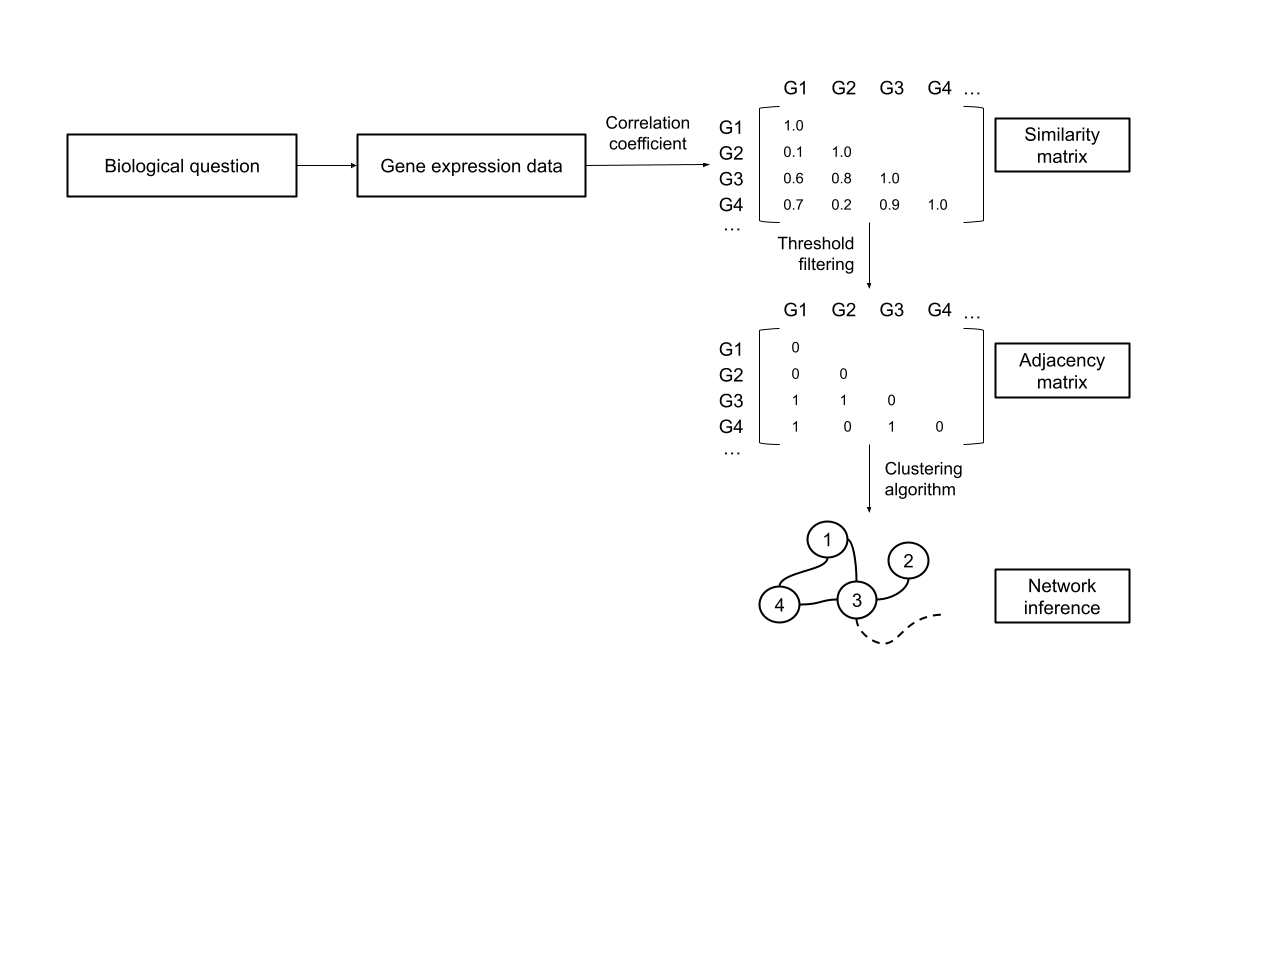
\includegraphics[width=1\linewidth]{Images/InDoc/networkProcess.png}
  \caption[Network Diagram]{\small Simplified representation of the process for network building. \textit{(Serin et al., 2016, p. 4)}}
    \label{fig:nwDg}
\end{figure}

\hypertarget{wgcna}{%
\subsection{WGCNA}\label{wgcna}}

To construct and analyze co-expression networks the most widely used
method is Weighted Gene Co-Expression Network Analysis (WGCNA). It is an
approach designed to identify gene modules and explore their relation
with phenotypic traits. Simple correlation-based networks use strict
thresholds to determine edges, while WGCNA constructs a weighted
network, where edges are assigned continuous values to reflect the
strength of the co-expression relationship. {(Langfelder \&
Horvath, 2008)}

WGCNA follows a series of steps to construct and analyze networks, the
process begins by using Pearson or Spearman correlations to compute the
pairwise correlation coefficients between gene expression profiles, with
those correlations an adjacency matrix is constructed. The matrix
quantifies the strength of the co-expression relationship between genes.

Next, a soft thresholding power is applied to the matrix to transform it
into a weighted network. This highlights strong correlations and
diminishes the influence of weaker associations, ensuring a better
reflection of underlying gene interactions and therefore an enhancement
in biologically important connections.

The network structure is further refined through the calculation of a
Topological Overlap Matrix (TOM), which takes into consideration
relationships between pairs of genes and the shared interactions that
happen with the whole network. This additional layer of connectivity
collaborates in the identification of biologically relevant clusters and
improves the robustness of the network.

Following the refinement of the co-expression network the genes are
grouped into similarly expressed modules, these modules are determined
by using hierarchical clustering and dynamic tree-cut algorithms and
represent sets of genes with highly similar expression patterns, which
suggests potential functional relationships.

Finally, the identified modules are correlated with external traits to
assess their biological significance and relations. Links can be
established using co-expression patterns and specific biological
processes by integrating variables such as tissues, developmental
stages, environmental conditions or phenotypic traits.

This also allows for the analysis of specific relations between modules,
and therefore genes, in detailed conditions or tissues, and also how a
concrete environmental condition might affect the whole transcriptome.

\hypertarget{maize-lines-and-transcriptional-variation}{%
\subsection{Maize lines and transcriptional
variation}\label{maize-lines-and-transcriptional-variation}}

Maize is a widely produced crop, one of the 3 most important plants
worldwide, it surpasses the global production of wheat and rice and has
become a staple food around the world, it has uses as human and animal
aliment, as a resource in industrial products and as a model organism in
genetics. The widespread cultivation of this crop is because it presents
a high yield potential, extensive genetic diversity and is extremely
adaptable. The mentioned genetic diversity is manifested in the
existence of multiple maize germplasms like Flour maize, Sweet maize,
Dent maize and Flint maize. Also the use of this diversity has been
extensively exploited in breeding programs to increase agronomic
efficiency, the most common method is inter-group hybridization, which
exploits heterosis for better yields.

This genetic diversity of maize has been well documented, pan-genome
studies present clear evidence of the multiple aspects that this crop
presents {(Haberer et al., 2020)}. However, the effect of this high genomic variability on the
transcriptional variation of different maize lines presents a lot of
research opportunities. Understanding the transcriptional diversity and
differences present in these lines is necessary for uncovering how
genetic differences have affected the regulation and functional pathways
causing the phenotypic variations into multiple maize lines. By
analysing gene co-expression networks that include multiple lines,
relationships can be found between gene expression, phenotypic traits
and differences in genome structure and organization.

To explore this, the present study focuses on five maize lines: B73,
DK150, EP1, F7 and PE75. B73 belongs to the U.S. Dent maize group is a
widely used reference genotype, for example, it serves as a benchmark
for comparative analysis. DK150, EP1 and F7 are all European Flint
lines, originating from southern Germany, northern Spain and southern
France. And PE75 is a derivation from a German landrace, the Petkuser
Ferdinand Rot population, a doubled-haploid line to represent a more
genetically diverse background.

A comprehensive transcriptome atlas was generated to capture expression
profiles across 30 tissues in the 5 maize lines, with multiple samples
per tissue for a better representation of the data. Tissues from
different zones of the plant and through multiple developmental stages
were chosen, like \emph{crown root}, \emph{cob}, \emph{leaf},
\emph{root} and \emph{seed}.

\begin{figure}[H]
  \centering
  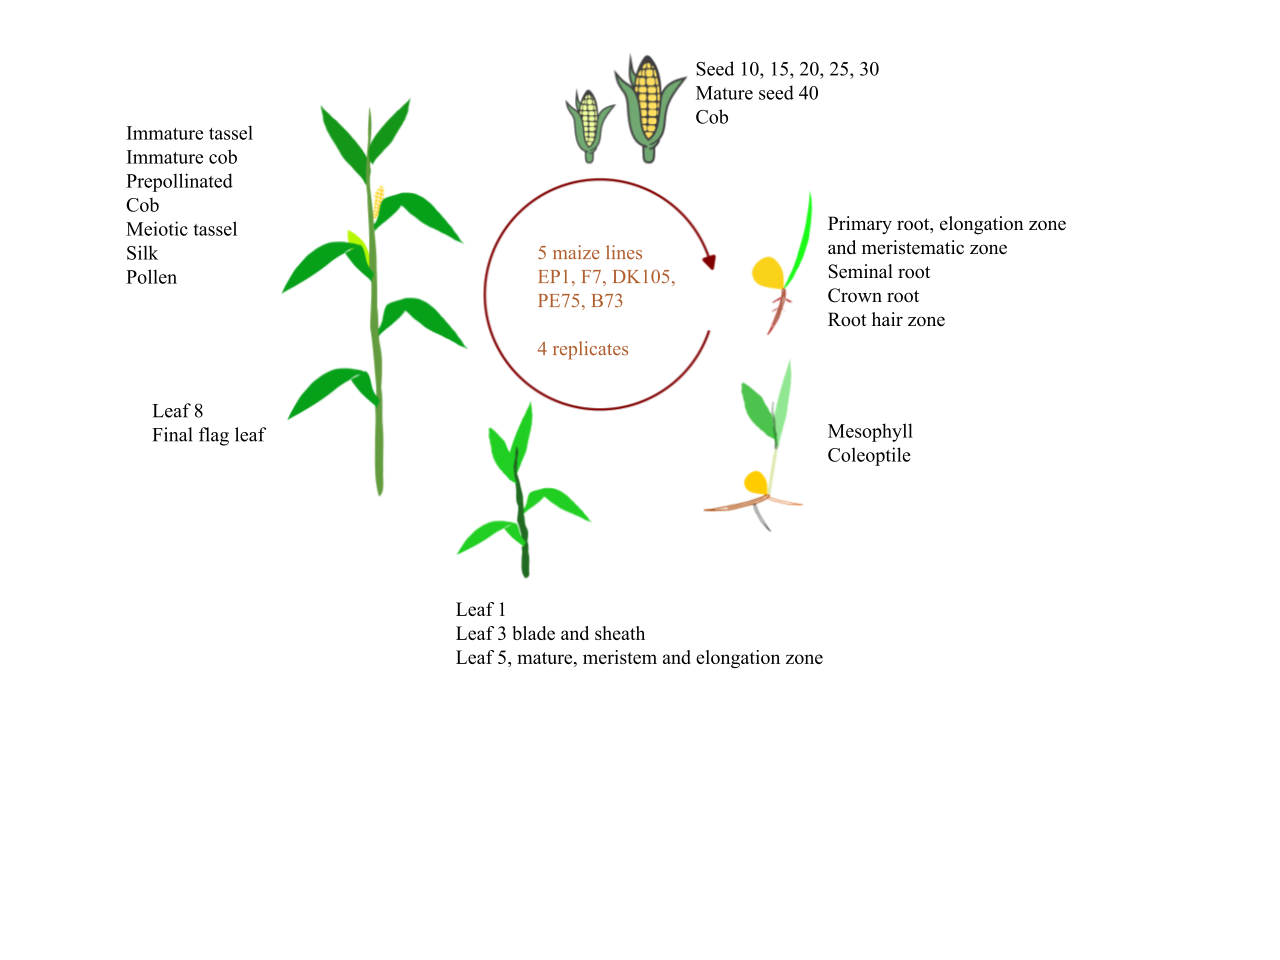
\includegraphics[width=1\linewidth]{Images/InDoc/Final_maizeCycle.png}
  \caption[Maize Cycle]{\small Representation of the stages and tissues where data from the 5 maize lines was gathered. (Image provided by Dr. Georg Haberer)}
    \label{fig:maize_cycle}
\end{figure}

This dataset contains the data for constructing genotype-specific gene
co-expression networks, enabling the creation of networks for
comparative analysis of transcriptional organization across different
genetic backgrounds. Using WGCNA, gene modules specific to each genotype
are separately examined for biological relevance. Using these
co-expression networks, the study intends to measure and determine the
amount of co-expression variance between genotypes, whether specific
functional modules are unique to certain genetic backgrounds, the
effects location may have had in the expression and therefore phenotype
development of these lines and how these differences reflect the
underlying regulatory mechanisms.

By integrating genotype-specific expression data in the co-expression
analysis, this research aims to contribute to a deeper understanding of
transcriptional regulation in maize and its relationship to genetic
diversity.

\hypertarget{objectives}{%
\section{Objectives}\label{objectives}}

This study intends to understand the relationship between the gene
expression patterns in 5 different maize lines and the phenotypic
differences they present by the employment of gene co-expression
networks.

An essential part of the study is to determine whether common gene
modules are present across the maize lines, how they relate to
phenotypic similarities, which modules are most common to be conserved
and to which phenotypic traits they relate. Complementary to this
objective, the study also aims to examine the diverging modules across
lines and uniqueness of modules, the transcriptional variations that
stem from these and their contribution to phenotypic divergence.

The ultimate goal of this research is to contribute to a broader
understanding of the maize transcriptome by offering insights into the
effect that gene expression has on genetic diversity. The finality that
it leads to is to provide a basis for further research on maize
breeding, genetic adaptation, and crop improvement.

\hypertarget{methods}{%
\section{Methods}\label{methods}}

\hypertarget{data-filtering}{%
\subsection{Data filtering}\label{data-filtering}}

The produced data and metadata contains errors and low quality samples,
it will need to be processed for cleaning. This process begins with an
evaluation of the metadata, where the quality of the samples is
assessed. Specifically, a quality score of 0 indicates high-quality
samples, while scores of 1, 2, or 3 denote progressively lower quality,
with 3 representing the poorest-quality samples. After careful
observation a discrepancy was identified between the number of samples
in the data and metadata, this can be tracked to samples belonging to
the pollen tissue, which are present in metadata but they have no
expression data. The lack of pollen samples in data is due to the
challenges associated with sequencing pollen tissue, from which not
enough genetic material could be extracted for successful sequencing.

To ensure consistency between gene expression data and metadata an R
script that removed any samples that were not present in both datasets
was used.

Subsequently, the renaming of a metadata column containing coded tissue
identifiers was executed using a python script, the objective was to
rewrite arbitrary numerical and alphanumeric codes with formalized
tissue abbreviations, for a better readability of the data. This
transformation was done by observing the data and creating a reference
dictionary, and systematically substituting each code by an
abbreviation.

Then the final step in the data preprocessing is to partition the data
into the different lines, as the intended analysis is a co-expression
analysis of traits within the individual species. The R script merges
the metadata with the gene expression data and subsequently divides the
dataset into separate tables for each species. After this, they are
split again into CSV and TXT files containing the expression data and
metadata for each maize line.

\hypertarget{replicates-in-the-data}{%
\subsection{Replicates in the data}\label{replicates-in-the-data}}

For all subsequent analyses, the data was processed separately for each
maize line. The first step involved removing outlier genes using WGCNA
module functions in R. This was done to remove data points which would
heavily skew our data while contributing minimal biological relevance.

Following this, the replicate samples for all tissues were merged to
address potential imbalances in the dataset. This was done to avoid bias
in the analysis caused by discrepancies in replicate numbers, as if
there were to be 4 replicates belonging to tissue \emph{silk} and only 1
belonging to tissue \emph{crown root}, that would skew the results. To
solve this imbalance the expression values for each gene across all
replicates of a given tissue were summed and then averaged by dividing
by the number of replicates, ensuring an equal contribution from all
replicates to the final dataset.

\hypertarget{normalization}{%
\subsection{Normalization}\label{normalization}}

To be able to extract conclusions from a counts table, normalization is
needed. The goal of normalization is to ensure that read counts
represent differences in true gene expression. This enables meaningful
comparisons across samples while reducing noise in the data, thereby
facilitating pattern recognition.

Normalization is crucial because raw gene expression values are not
inherently comparable between samples, the total number of reads can
vary across samples and so a large difference in a gene's read count
between different conditions may simply be the result of differential
coverage.

Raw gene expression comparisons are also affected by random variability
in the alignment to a given gene within a specific sample. Additionally,
normalization is needed because it also accounts for variations in the
total RNA content across samples, ensuring their compatibility for
comparison.

\begin{figure}[H]
  \centering
  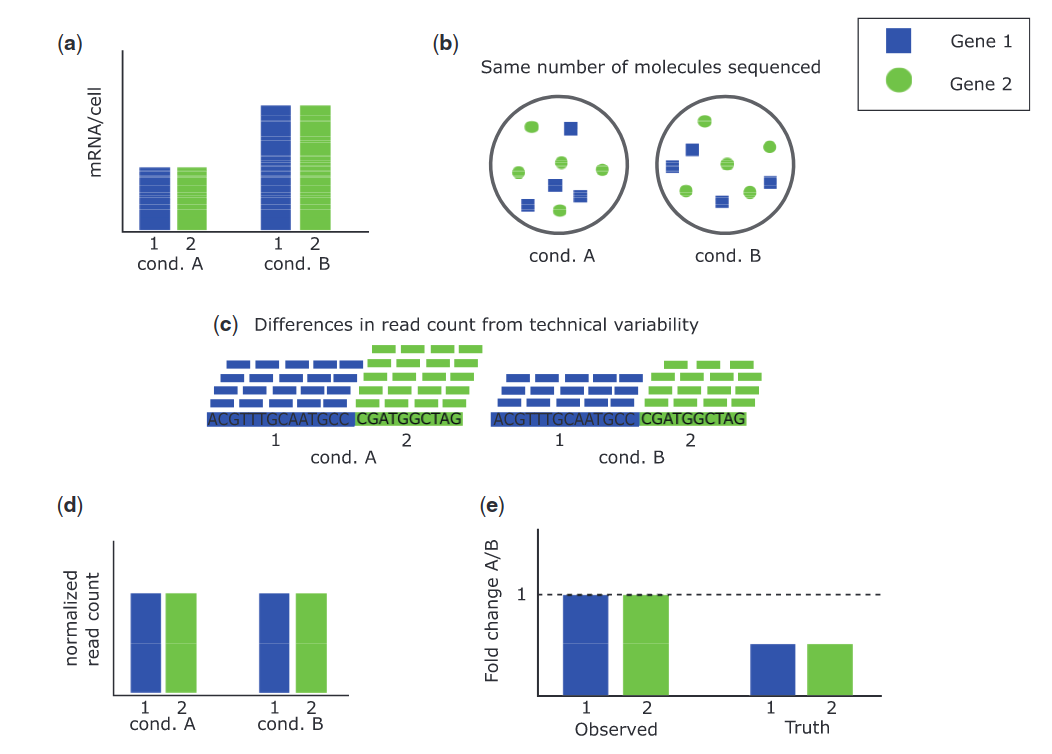
\includegraphics[width=1\linewidth]{Images/InDoc/EvansHall_normalization.png}
  \caption[Normalization assumptions]{\small 
  	Two genes, and an experiment to compare expression between
	condition A and condition B. \textbf{(A)} Global up-regulation under
	condition B for both genes, the same amount of mRNA/cell is produced.
	\textbf{(B)} Same number of molecules sequenced under the 2 conditions,
	and the two genes produce the same amount of mRNA, as gene 2 is
	four-fifths the length of gene 1, so it must produce five-fourths the
	number of molecules that gene 1 does. \textbf{(C)} Sequenced reads are
	aligned to the reference genome and mapped to each gene. The
	distribution of reads is the same in each sample, but by chance the
	sample for condition A happens to have more reads in total. \textbf{(D)}
	A normalization process is executed, it removes the differences in read
	count from technical variability, which stabilizes the counts for the
	genes in both conditions. \textbf{(E)} In (D) the normalized read counts
	are the same, the observed fold change for each gene is 1, indicating no
	differential expression. However, the genes are twice as expressed under
	condition B, so we should observe half the expression when comparing A
	to B. \textit{(Evans et al., 2017, p. 4)}
  } %caption end
    \label{fig:norm_ass}
\end{figure}

There are multiple approaches to data normalization: by library size, by
control genes and distribution-based methods. Each of these approaches
relies on a specific parameter such as gene length or a gene group as
reference. Moreover, different assumptions are made for each approach,
therefore choosing the right approach is key, as wrong assumptions can
lead to erroneous results as shown in Figure \ref{fig:norm_ass}. In this study,
normalization was performed by library size, more concretely using these
2 methods: Reads Per Kilobase per Million mapped reads (RPKM) and Counts
Per Million (CPM), which were both used and subsequently compared
against each other to determine the most suitable approach..

The RPKM method accounts for gene length and sequencing depth but may be
biased by RNA composition differences. Additionally, it is not ideal for
cross-sample comparisons. And CPM is a method that adjusts only for
sequencing depth and performs well when comparing samples with similar
composition. However, in CPM normalization longer genes may appear more
highly expressed.

To select the appropriate method, the dataset was processed using both
methods and the results were evaluated. The program hinges on the edgeR
R package to provide the normalization and it uses the same process to
apply a logarithmic transformation to the data. The distribution of
normalized values was then visualized graphically for each method to
assess its effectiveness.

\begin{figure}[H]
  \centering
  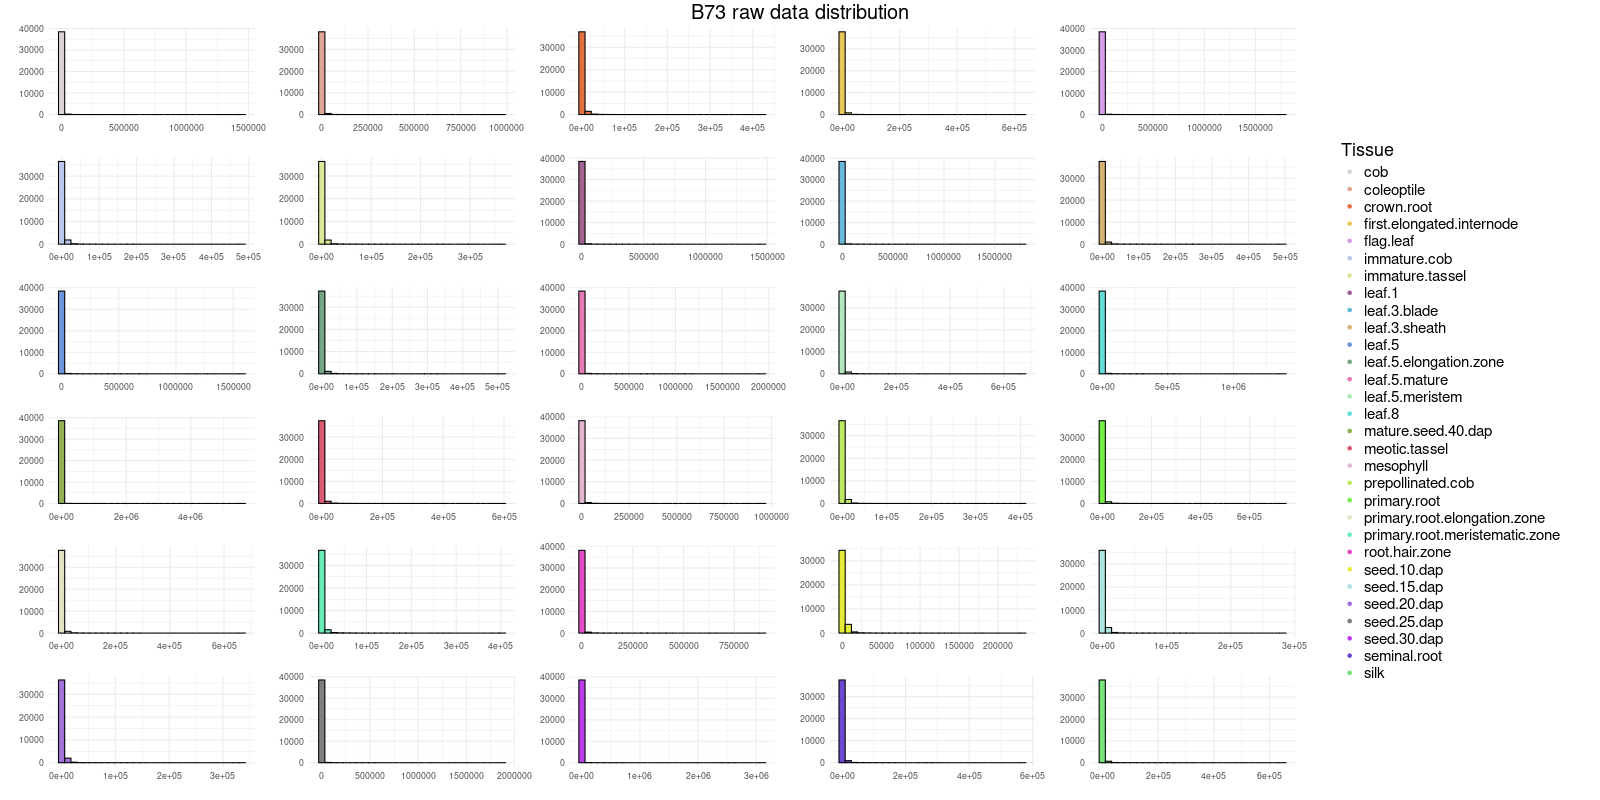
\includegraphics[width=1\linewidth]{Images/InDoc/B73_raw_distPlot.png}
  \caption[B73 raw distribution]{\small Plot of the distribution of the gene expression data for all tissues of maize line B73 with no normalization.}
    \label{fig:raw_Dist}
\end{figure}

Figure \ref{fig:raw_Dist} is raw data distribution, it can be seen that most genes
present the expression at similar, very low, levels, if the data is
normalized the visualization will be better.

\begin{figure}[H]
  \centering
  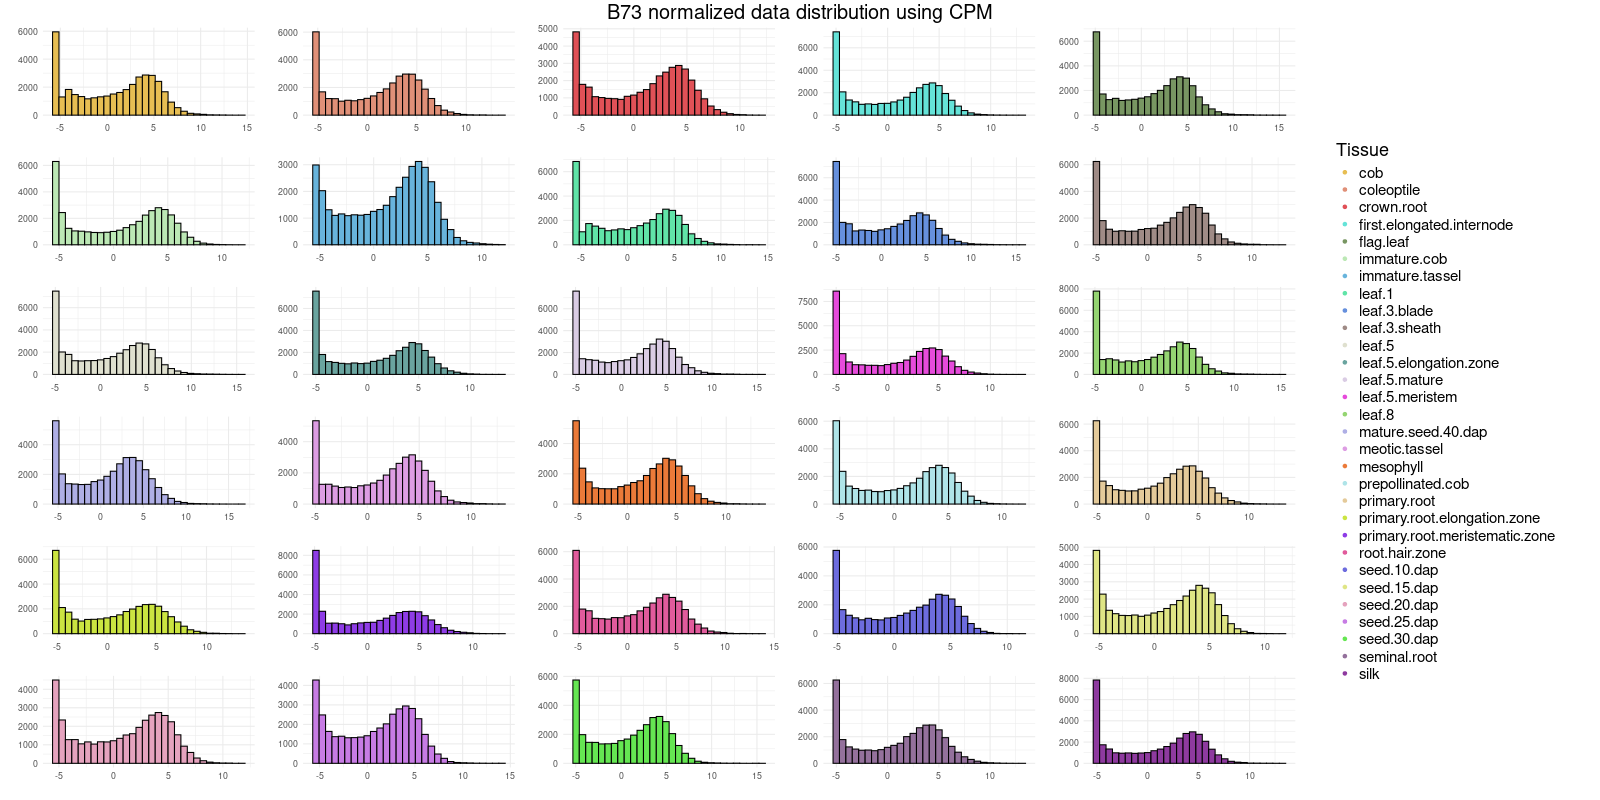
\includegraphics[width=1\linewidth]{Images/InDoc/unf-B73_normCPM_distPlot.png}
  \caption[B73 CPM distribution]{\small Plot of the distribution of the gene expression data for all tissues of maize line B73 where CPM normalization was performed using edgeR.}
    \label{fig:CPM_Dist}
\end{figure}

In Figure \ref{fig:CPM_Dist} the data has been normalized using CPM, however, an
anomaly can be observed in the distribution, an extreme increase in low
expression representation which means that the data is not correctly
normalized. The resulting distribution appears to be a bimodal
distribution, with an irregular peak present in the region of low
expressed genes.

\begin{figure}[H]
  \centering
  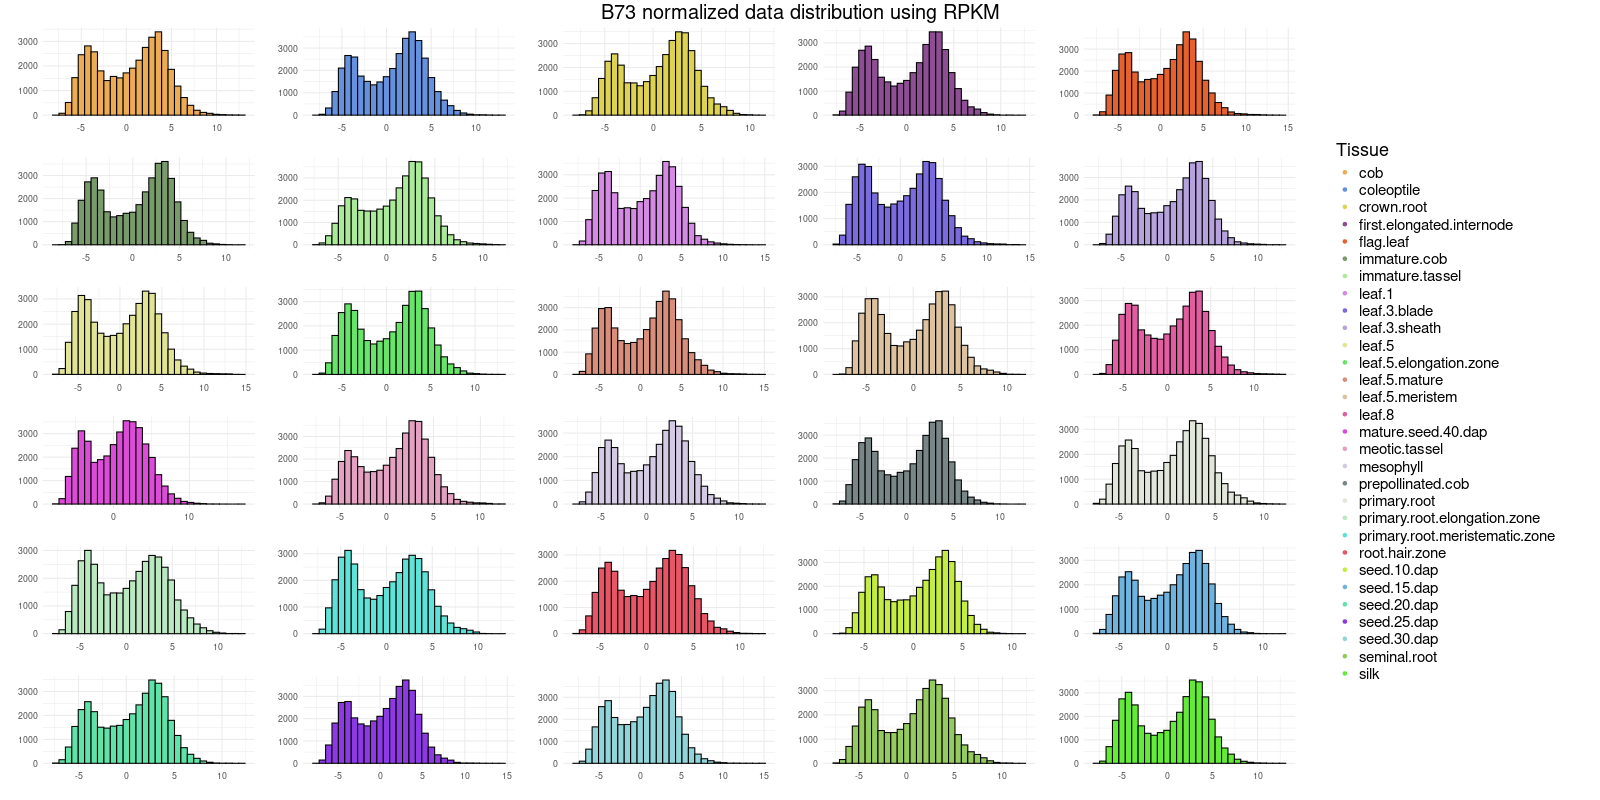
\includegraphics[width=1\linewidth]{Images/InDoc/unf-B73_normRPKM_distPlot.png}
  \caption[B73 RPKM distribution]{\small Plot of the distribution of the gene expression data for all tissues of maize line B73 where RPKM normalization was performed using edgeR.}
    \label{fig:RPKM_Dist}
\end{figure}

The Figure \ref{fig:RPKM_Dist} graph represents RPKM-normalized data, which should
ideally follow a normal distribution in the shape of a bell curve.
However, it can be observed that this is not the case. Instead the plots
exhibit a bimodal distribution, with an irregular peak corresponding to
the low expressed genes.

In both normalized data graphs anomalies can be observed due to
overrepresentation of lowly expressed genes. To achieve a completely
normalized data, the lowly expressed genes must be removed. Removing the
lowly expressed genes is done through gene expression filtering.

\hypertarget{filtering-of-lowly-expressed-genes}{%
\subsection{Filtering of lowly expressed
genes}\label{filtering-of-lowly-expressed-genes}}

Filtering by gene expression is an essential step in the workflow as it
eliminates background noise caused by lowly expressed genes. The removal
of lowly expressed genes is a useful procedure because it enhances
Differentially Expressed Gene (DEG) detection sensitivity, improving
later analysis. The initial stage of the workflow is evaluating the
impact of expression filtering in the 2 normalization processes and
comparing the number of genes retained in each case.

A consistent filtering strategy is applied across both methods, wherein
the total counts of each gene whose individual count is higher than a
predefined threshold (\emph{x)} are summed, and only those with a total
count equal to or greater than a predefined threshold (\emph{y}) are
retained. These threshold values (\emph{x} and \emph{y}) differ
depending on the normalization method to allow for an optimal
normalization. The values and retained genes while maintaining a normal
distribution are:

\begin{longtable}[]{@{}c c c c@{}}
\toprule
\textbf{} & \emph{\textbf{x}} & \emph{\textbf{y}} & \textbf{genes kept/total genes} \tabularnewline
\midrule
\endhead
\textbf{CPM} & 1 & 12 & 22205/38708 \tabularnewline
\textbf{RPKM} & 0 & 10 & 24537/38708 \tabularnewline
\bottomrule
\end{longtable}


%CPM and RPKM TC normalization figures
\begin{figure}[H]
  \centering
  
  	\subfloat {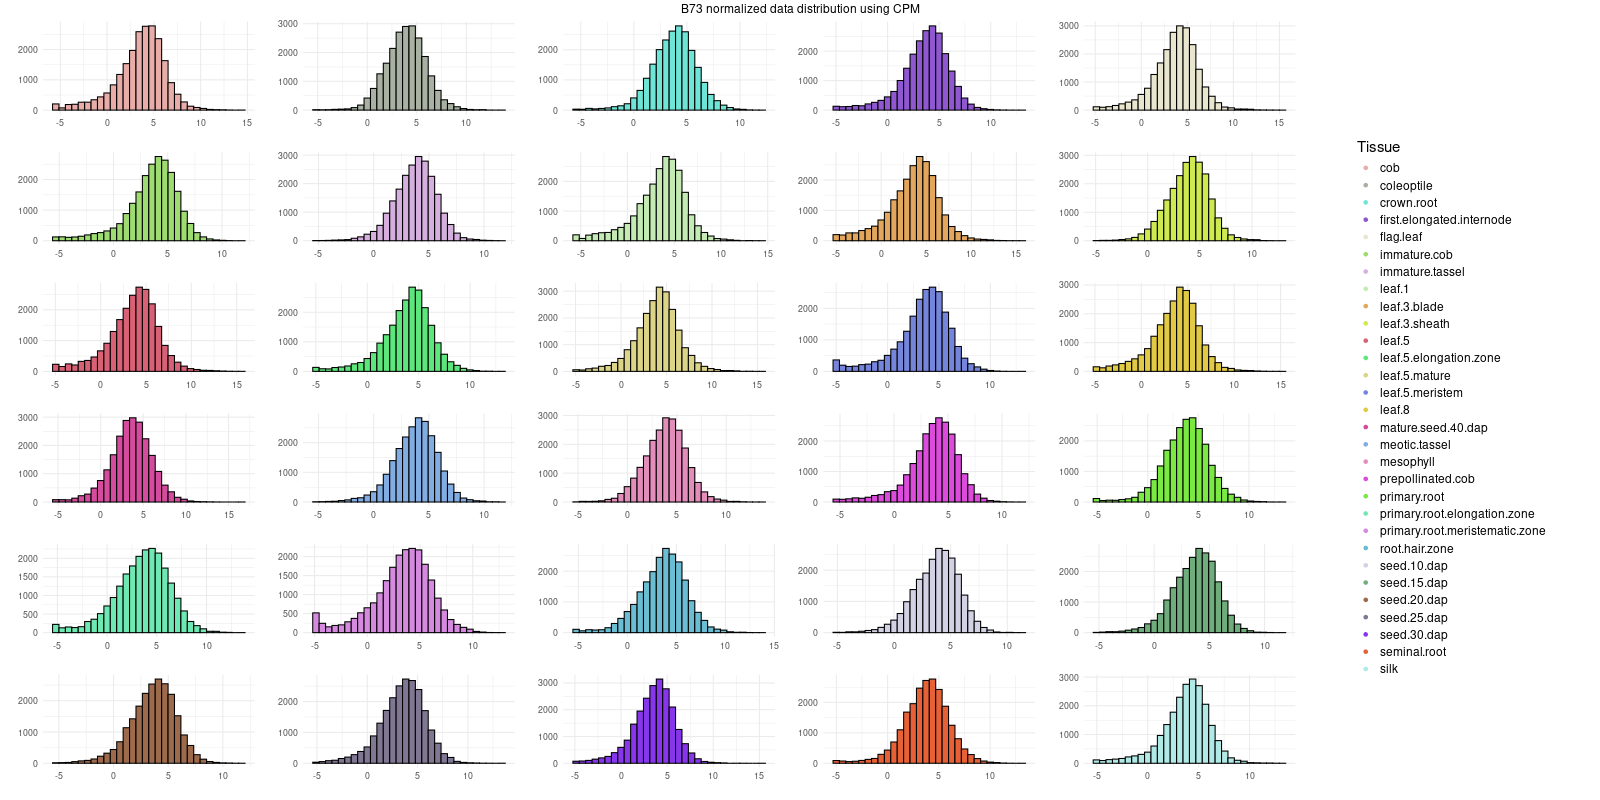
\includegraphics[width=1\linewidth]{Images/InDoc/B73_normCPM_distPlot.png} \label{fig:TCfilterCPM_Dis}} \\
  	\subfloat {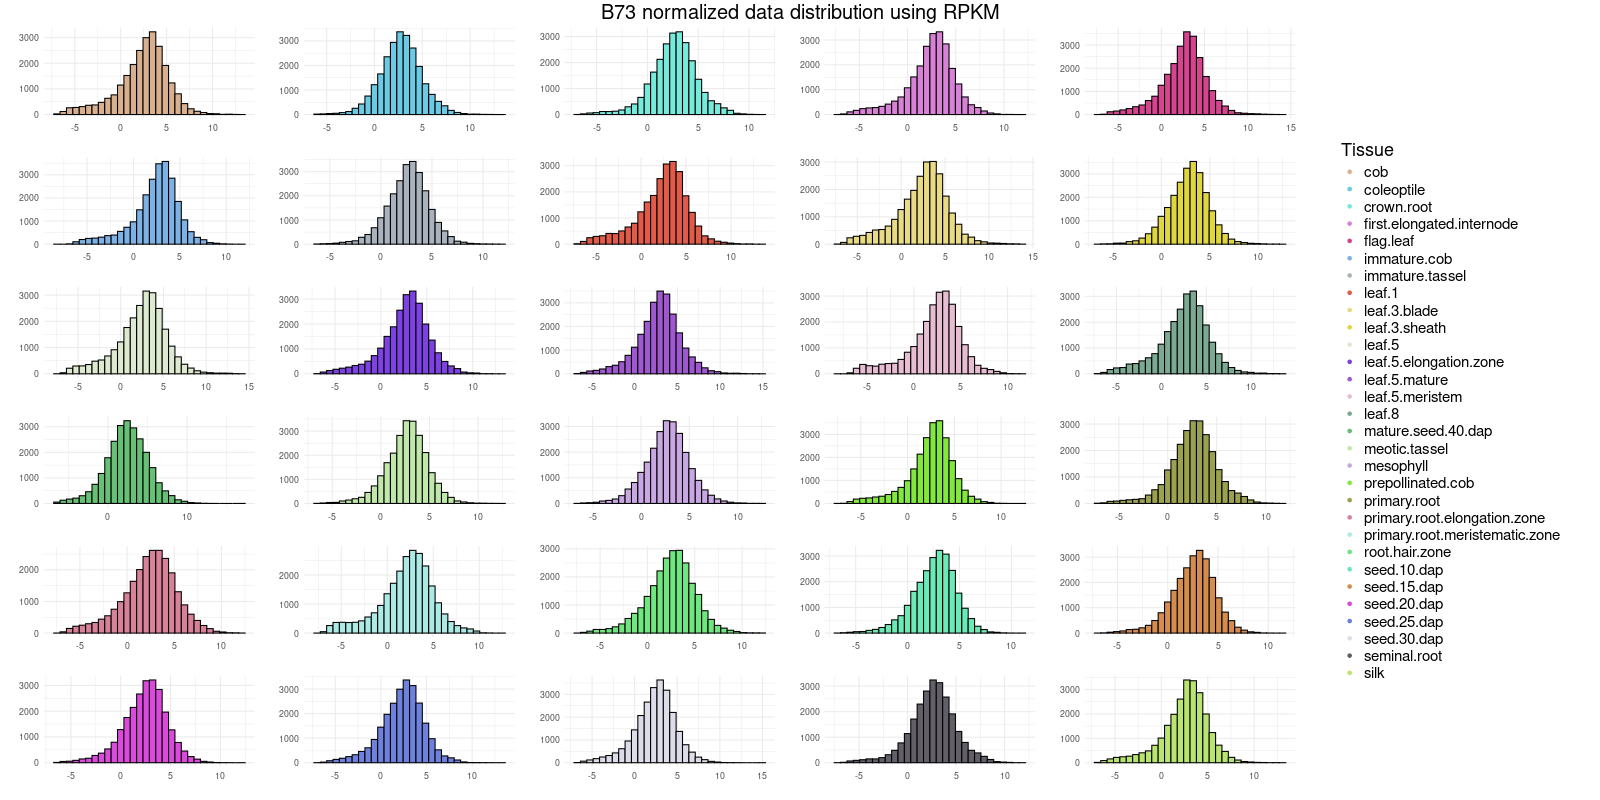
\includegraphics[width=1\linewidth]{Images/InDoc/B73_normRPKM_distPlot.png} \label{fig:TCfilterRPKM_Dis}}
  	
  \caption[Filter TC B73 distribution]{\small Plot of the distribution of the gene expression data for all tissues of maize line 
  B73 where CPM or RPKM normalization and gene filtering through total counts have been performed.} %caption
  \label{fig:TCfilter_Dis}
\end{figure}


In the plots represented in Figure \ref{fig:TCfilter_Dis} it is evident that the data
distribution is almost identical to that of a normal distribution in
both methods, even though some slight variations are present in
particular cases of both CPM and RPKM. For all subsequent analysis it
must be assumed that RPKM will be used, as it produces similar results
than CPM while retaining a much larger content of genes.

After evaluating the filtering based on total gene count an alternative
method was proposed. Filtering only by total count may overlook cases
where a gene is highly represented in a single sample, potentially
missing important correlations. To address this issue, the new approach
combines filtering by total gene count, as in the previous method, with
an additional criterion: retaining genes that exhibit at least a value
greater than a predetermined threshold \emph{t}, even if the total of
the gene is not greater than the predefined threshold.

To assess the effectiveness of this method, both the fitness of the data
distribution and the number of retained genes are considered. The
thresholds \emph{x}, \emph{y} and \emph{t} vary depending on the methods
used to allow for the most optimal normalization, considering that the
distributions are similar in both cases, this figure illustrates the
differences they produce on the amount of retained genes.

\begin{longtable}[]{@{}c c c c c@{}}
\toprule
& \emph{\textbf{x}} & \emph{\textbf{y}} & \emph{\textbf{t}} &
\textbf{genes kept/total genes}\tabularnewline
\midrule
\endhead
\textbf{CPM} & 1 & 12 & 8 & 22654/38708\tabularnewline
\textbf{RPKM} & 0 & 10 & 6 & 25296/38708\tabularnewline
\bottomrule
\end{longtable}

%CPM and RPKM TC normalization figures
\begin{figure}[H]
  \centering
  
  	\subfloat {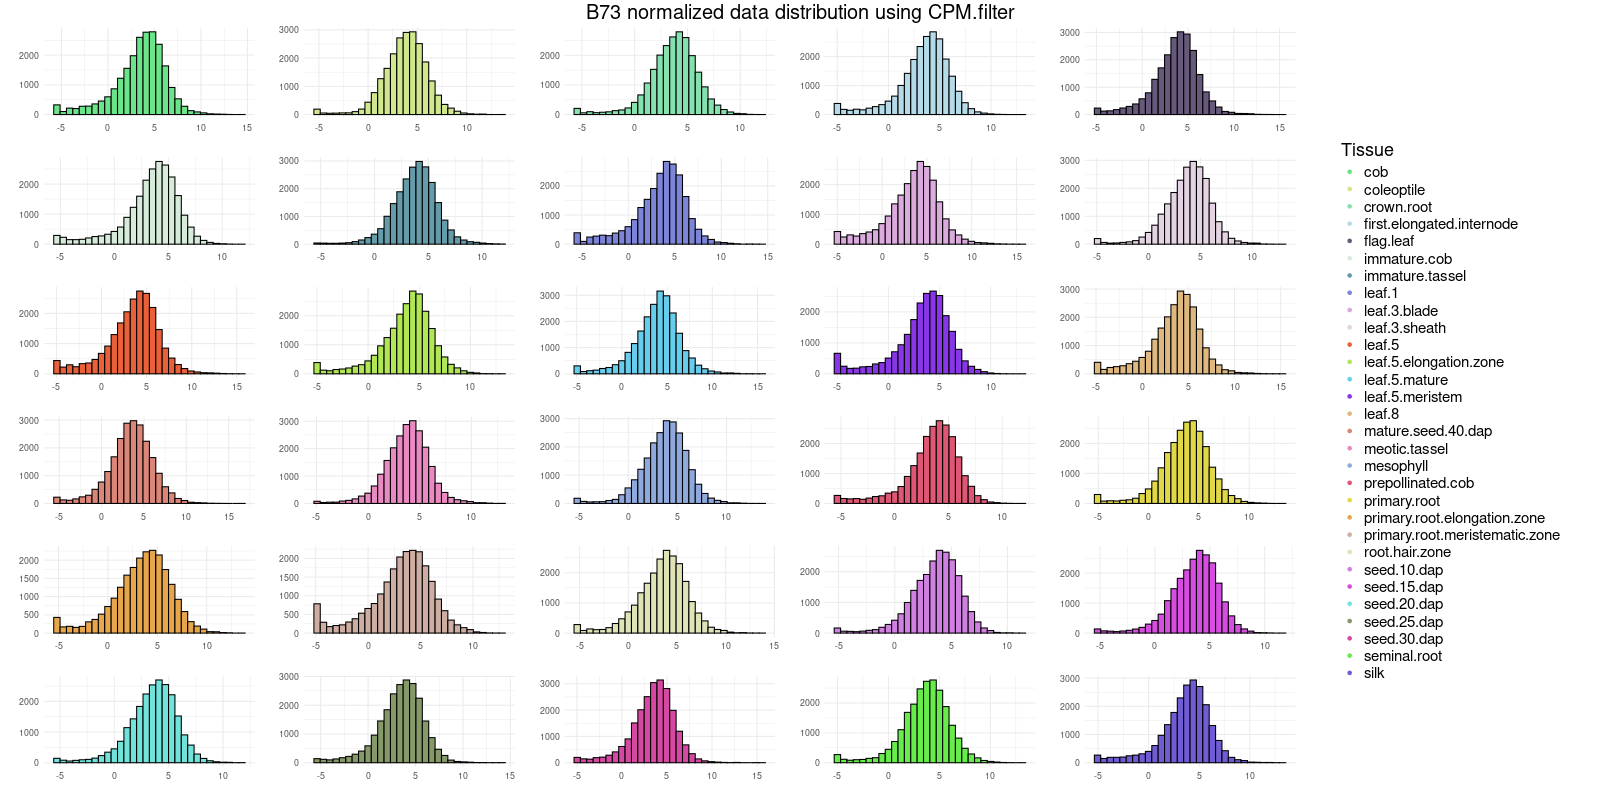
\includegraphics[width=1\linewidth]{Images/InDoc/B73_normCPM.filter_distPlot.png} \label{fig:SCfilterCPM_Dist}} \\
  	\subfloat {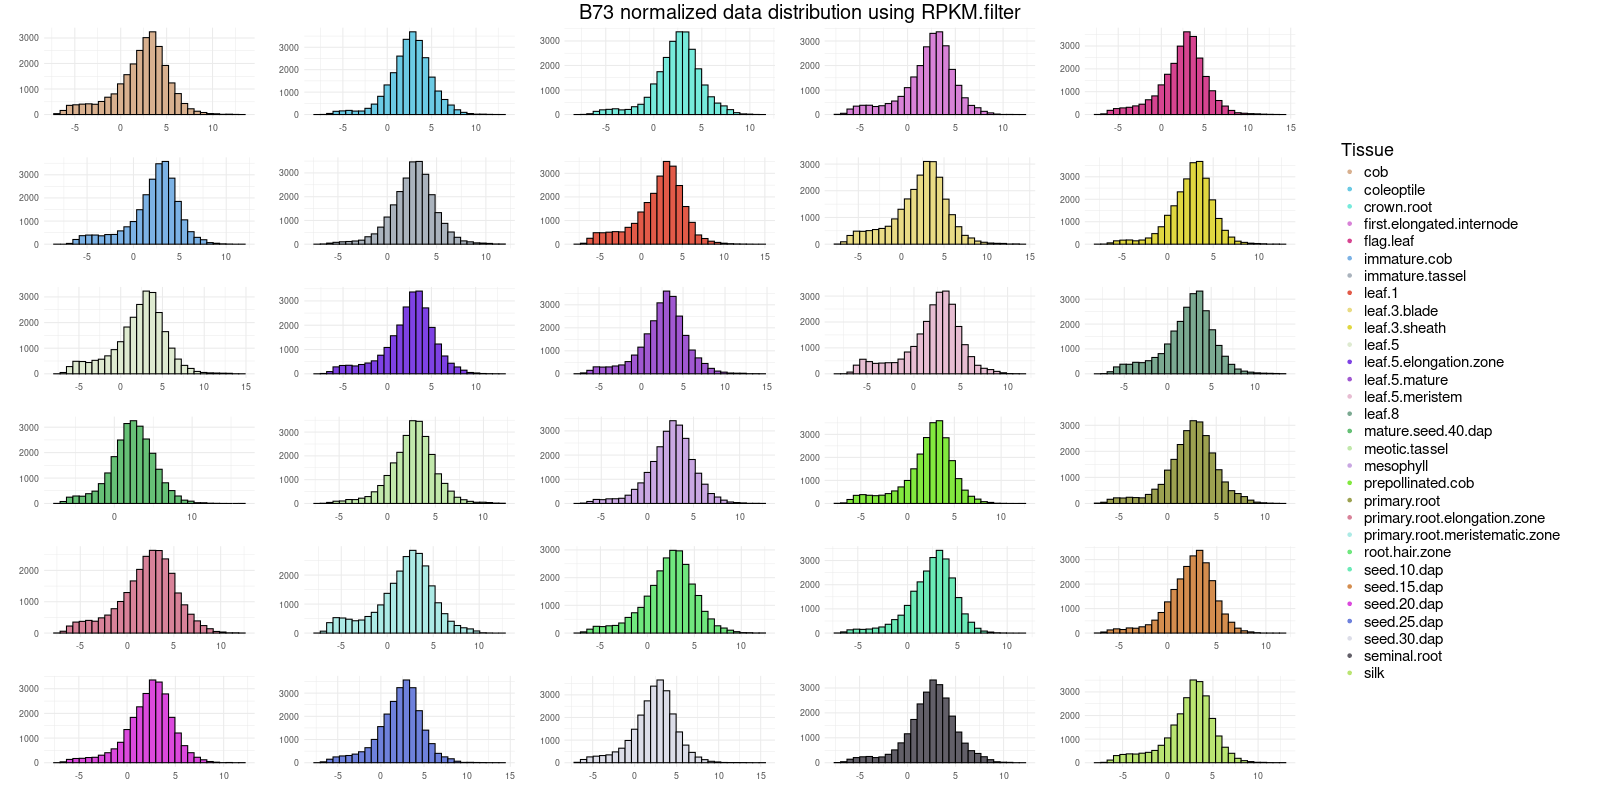
\includegraphics[width=1\linewidth]{Images/InDoc/B73_normRPKM.filter_distPlot.png} \label{fig:SCfilterRPKM_Dist}}
  	
  \caption[Filter SC B73 distribution]{\small Plot of the distribution of the gene expression data for all tissues of maize line B73 
  where CPM or RPKM normalization and gene filtering through sample counts have been performed.} %caption
  \label{fig:SCfilter_Dist}
\end{figure}

The graphs represented in Figure \ref{fig:SCfilter_Dist} demonstrate that both CPM and RPKM
exhibit similar distributions. However, RPKM aligns more closely with a
normal distribution and retains a greater set of genes. This finding is
consistent with the conclusions drawn from the filtering by total counts
method. As a result, all subsequent analysis will be conducted using the
RPKM data, filtered by this second method as it retains a larger amount
of genes.

\hypertarget{network-construction-and-gene-clustering}{%
\subsection{Network construction and gene
clustering}\label{network-construction-and-gene-clustering}}

Following the filtration process, the next step in constructing the gene
co-expression network involves clustering genes while maintaining an
appropriate soft-thresholding power, which will vary for each data set.
To determine the appropriate power for each case, the program considers
the signed R\textsuperscript{2} and the mean connectivity, selecting the
optimal value from a range of 1 to 17 and odd numbers between 17 and 49.
If the value exceeds 30 it is capped, as that is the maximum soft power
allowed for clustering.

The gene clustering process is performed with the WGCNA function
"blockwiseModules". This function requires the specification of a block
size, which is set to a value greater than the genes, provided that the
system memory permits it. This approach allows for processing as a
single block, thereby enhancing the clustering quality, ensuring a more
comprehensive network representation. The procedure employs a high deep
split parameter and signed TOM type, coupled with a low mergeCutHeight
for a highly sensitive module detection with substantial, though not
extreme, granularity. The resulting gene clusters vary in number across
the different maize lines, reflecting distinct expression pattern
associations.

Genes that do not fit into any specific cluster are assigned to the grey
module, a category for unclassified genes. For the quantity of genes in
our samples, the module is ideally maintained at a 1000 genes maximum.
Key parameters that influence the regulation of this module's size
include the initial normalization and filtering methods, which ensure
high-quality input data and sufficient gene retention for optimal
clustering, the blockwiseModules parameters, which enhance granularity
and classification accuracy, and finally, the soft-thresholding power
selection, as it impacts the overall network structure.

An adjacency table is generated from the replicate data. This table in
conjunction with the gene expression dataset is the object utilized to
calculate the correlations between the gene modules and replicates, and
enables the downstream analysis of module-trait relationships.

\hypertarget{preliminary-results}{%
\section{Preliminary results}\label{preliminary-results}}

The final product of the co-expression analysis is the correlation of an
adjacency table which contains the gene expression grouped by modules
and the traits that are to be analyzed. For the visualization of these
relations a correlation plot that includes the significance of the cases
is processed for each line.

\begin{figure}[H]
  \centering
  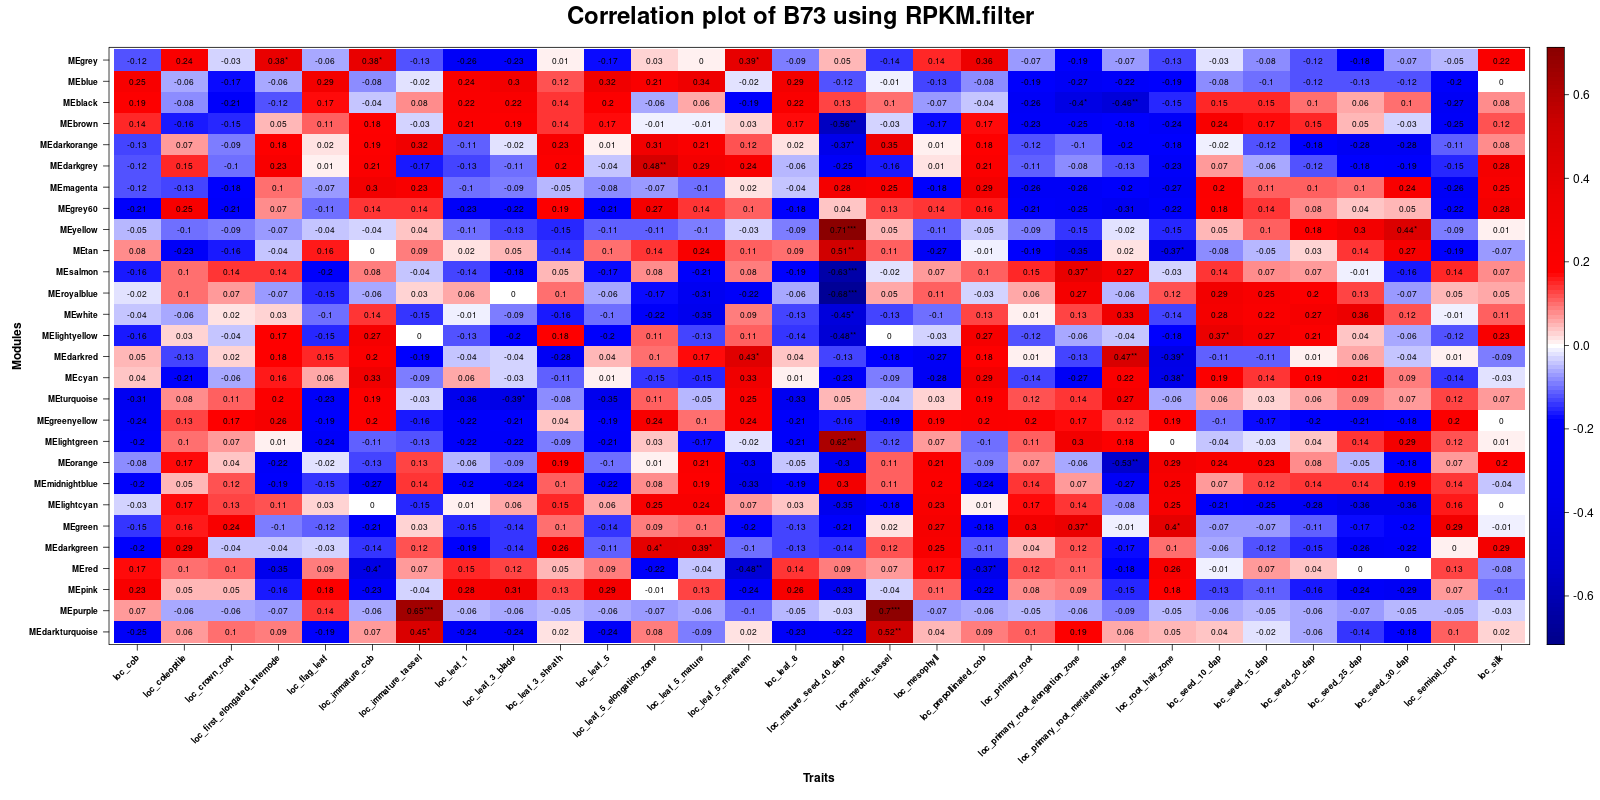
\includegraphics[width=1\linewidth]{Images/CorPlots/filtered/B73_RPKM.filter_corplot.png}
  \caption[B73 Correlation Plot]{\small Representation of module-trait relationships in the B73 maize line.}
    \label{fig:B73_CorPlot}
\end{figure}

On Figure \ref{fig:B73_CorPlot} clear functional groups of gene modules can be identified,
at a first glance the observation can be made that MEsalmon, MEblue,
MEred, MEgreenyellow, MEroyalblue and ME lightgreen are all involved in
up-regulation on root tissues, while ME turquoise, MEtan, MEgrey60,
MEcyan, MElightcyan and MEblack are involved in root tissues as well,
but in suppressed expression.

There are 4 modules which appear to be heavily involved in the early
stages of the leaf growth process.

Most seed traits share MEgreenyellow, MEroyalblue as down-regulated
modules, while 5 modules appear up-regulated, MEblack is predominant in
later seed stages and MElightyellow and MEgreen are heavily involved in
early stages. Most modules that appear in seed development genes appear
differentially expressed in root regulatory genes as well, but appear in
opposite regulatory patterns.

\begin{figure}[H]
  \centering
  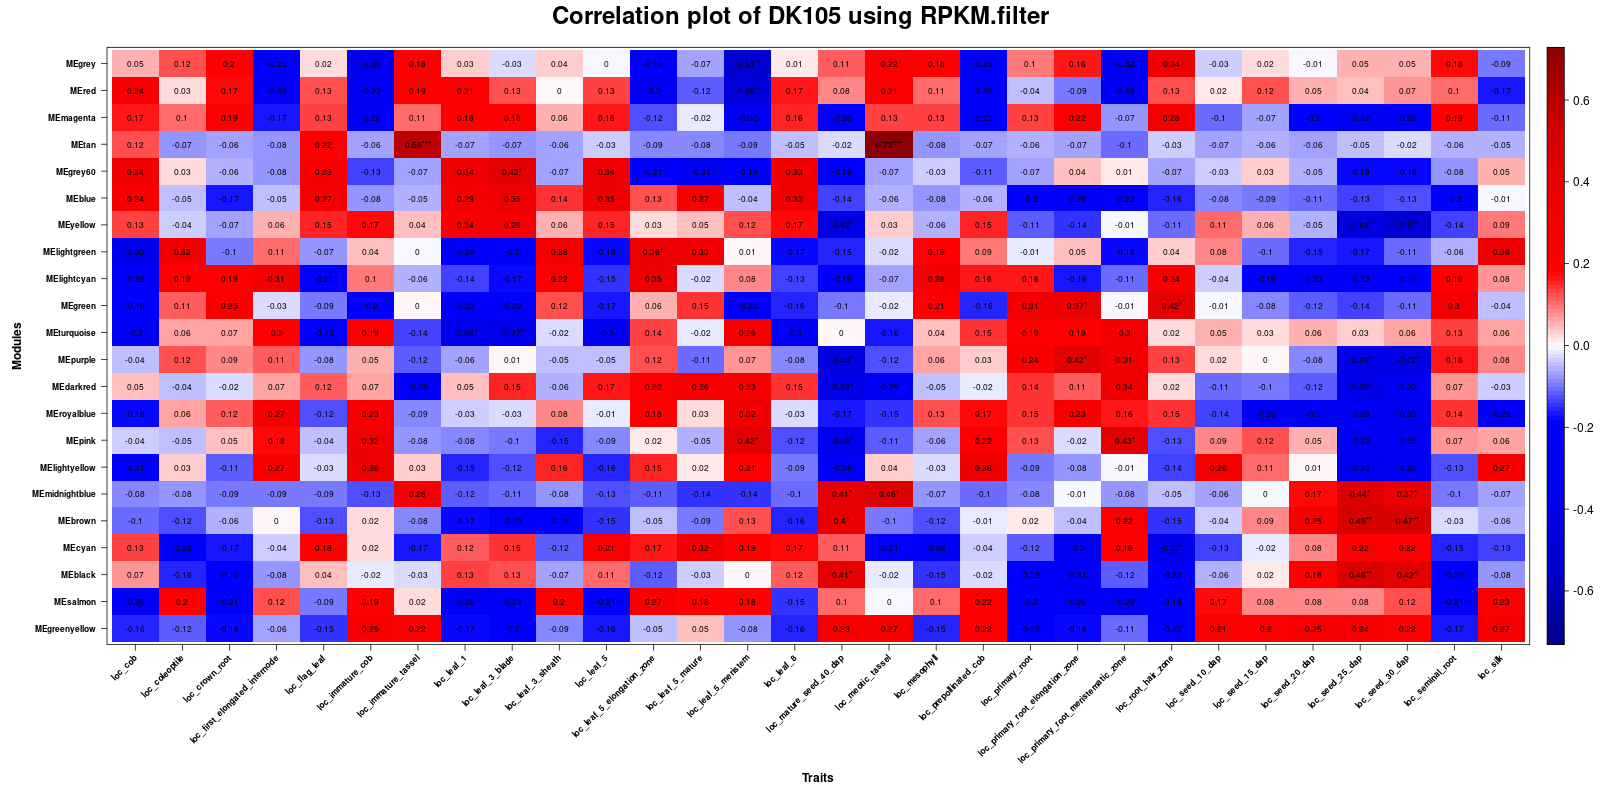
\includegraphics[width=1\linewidth]{Images/CorPlots/filtered/DK105_RPKM.filter_corplot.png}
  \caption[DK105 Correlation Plot]{\small Representation of module-trait relationships in the DK105 maize line.}
    \label{fig:DK105_CorPlot}
\end{figure}

In the correlation plot of DK105, which can be observed in Figure \ref{fig:DK105_CorPlot}, a
clear gene module to trait relation is between 13 gene modules and the
late stages of seed development, where a majority appear as
down-regulated modules. Out of these 13 gene modules MEcyan, MEsalmon
and MEgreenyellow are also relevant in the early stages of seed
development.

There are also strong co-expression patterns that identify the clear
involvement of 8 modules in primary root development, of these modules
the suppressed ones are also over expressed in late-stage seed
development, presenting a possible relation between the traits.

\begin{figure}[H]
  \centering
  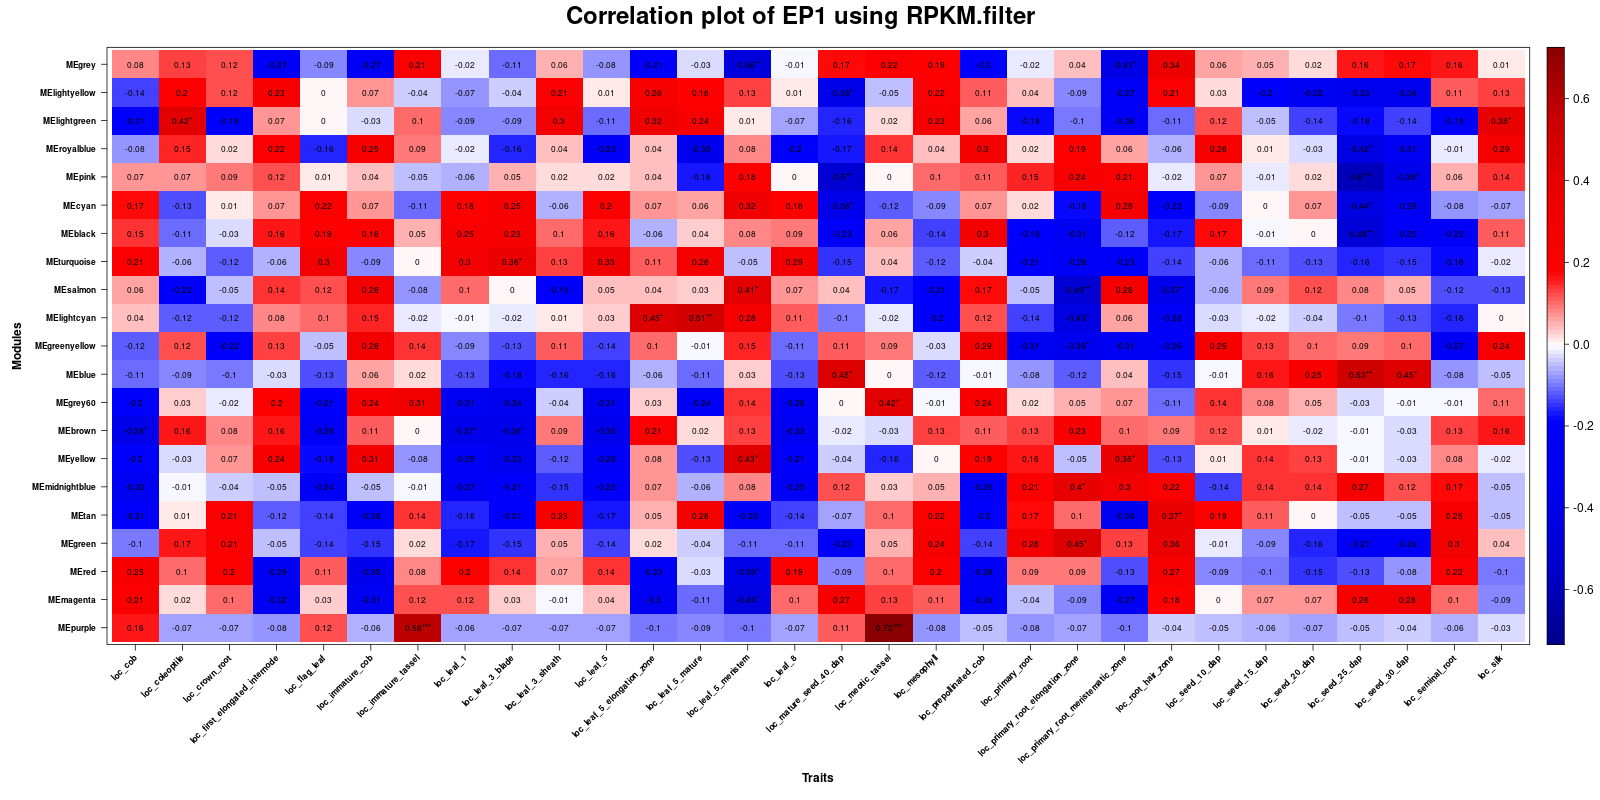
\includegraphics[width=1\linewidth]{Images/CorPlots/filtered/EP1_RPKM.filter_corplot.png}
  \caption[EP1 Correlation Plot]{\small Representation of module-trait relationships in the EP1 maize line.}
    \label{fig:EP1_CorPlot}
\end{figure}

In Figure \ref{fig:EP1_CorPlot} which corresponds to the correlation plot of EP1 genotype
it can be observed that usual expression patterns can not be observed,
most other maize lines show clear up-regulation patterns in seed
development traits, while in EP1, only 3 significantly up-regulated
modules are present, while 8 appear suppressed mainly in late stage
development modules. There is a clear differential expression in leaf
traits, specifically in the earliest and latest stages of development,
where 10 modules tend to be significantly expressed, 7 of them
suppressed while MEcyan, MEblack and MEturquoise are overexpressed. In
root development, 12 modules seem to be differentially expressed, most
appear as down-regulated, however, the patterns that can be observed in
other lines between seed and root development are missing.

\begin{figure}[H]
  \centering
  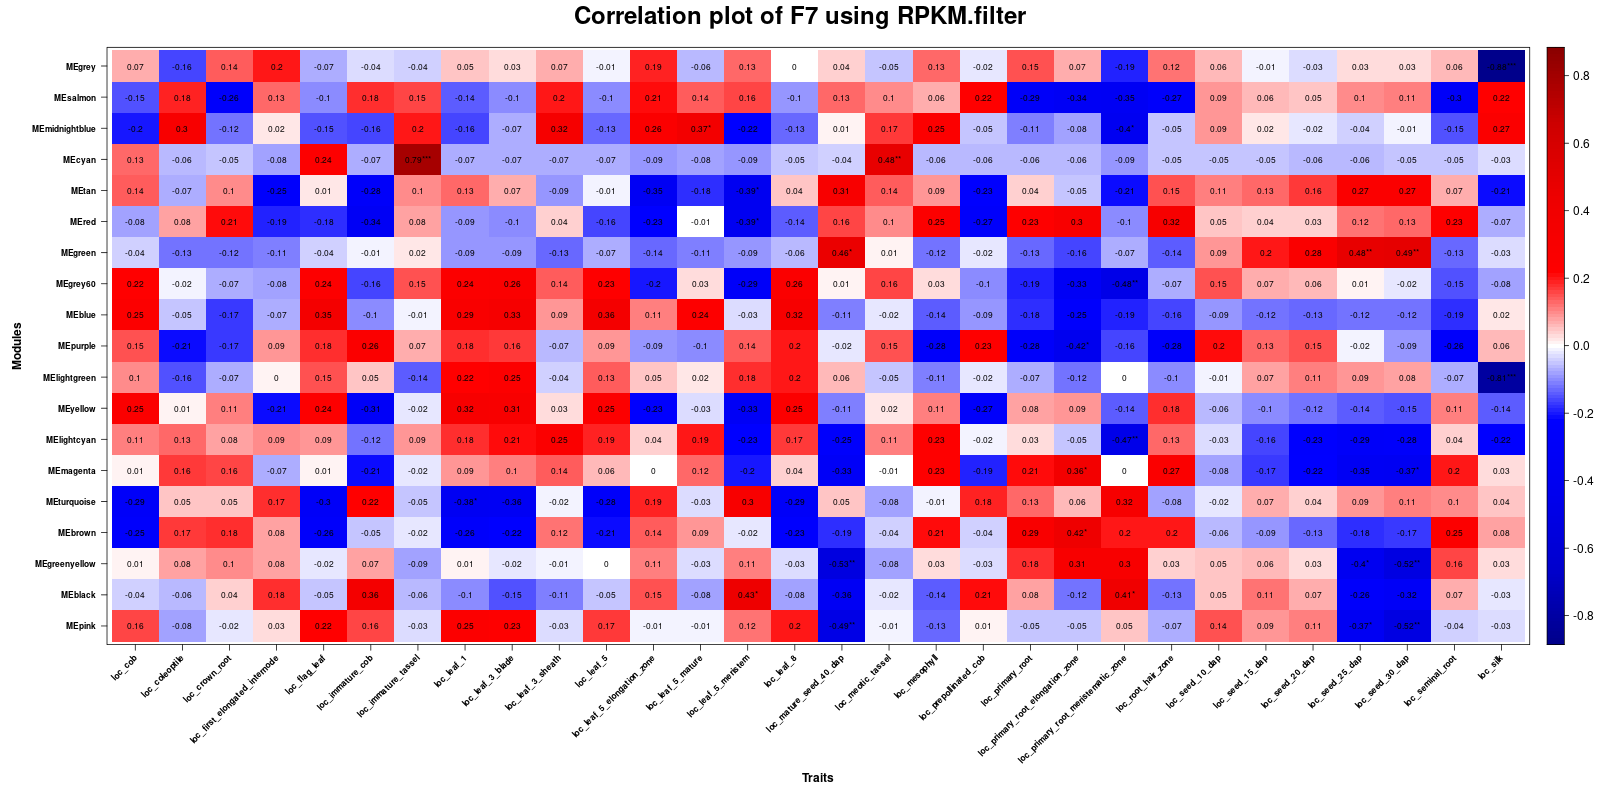
\includegraphics[width=1\linewidth]{Images/CorPlots/filtered/F7_RPKM.filter_corplot.png}
  \caption[F7 Correlation Plot]{\small Representation of module-trait relationships in the F7 maize line.}
    \label{fig:F7_CorPlot}
\end{figure}

According to Figure \ref{fig:F7_CorPlot} expression patterns in the F7 genotype are very
similar to those present in EP1, it presents a lack of up-regulated seed
trait modules, as well as strong differential expression on the root and
leaf traits. The differences are that in leaf traits more genes are
overexpressed than in the EP1 genotype and in the root traits there is a
stronger differential expression as well as more representation of
up-regulated modules. Also, in this maize line the expression patterns
present in most lines between root and seed are missing as well.

\begin{figure}[H]
  \centering
  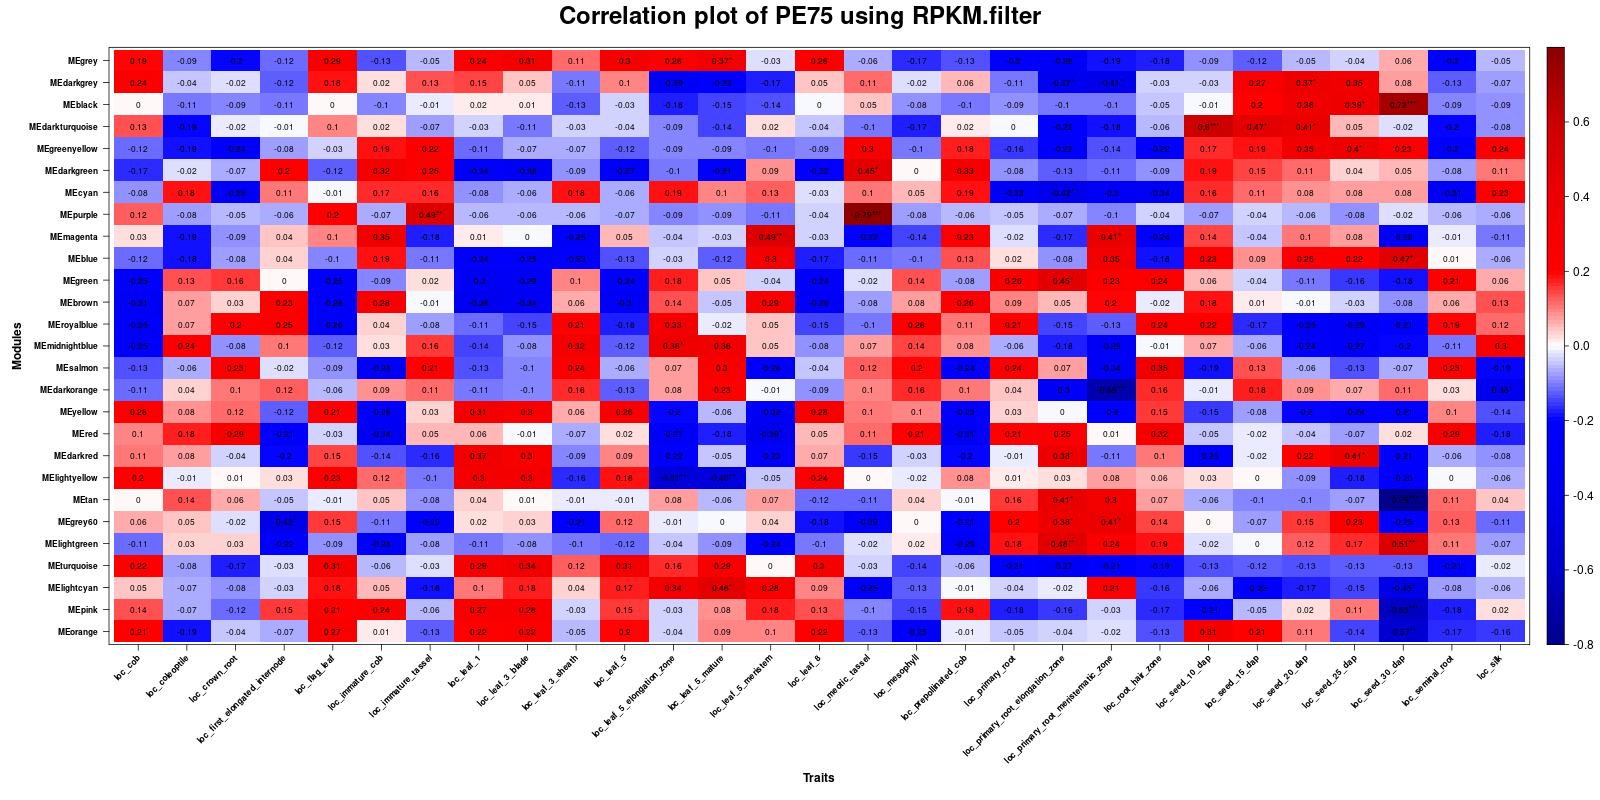
\includegraphics[width=1\linewidth]{Images/CorPlots/filtered/PE75_RPKM.filter_corplot.png}
  \caption[PE75 Correlation Plot]{\small Representation of module-trait relationships in the PE75 maize line.}
    \label{fig:PE75_CorPlot}
\end{figure}

Observing Figure \ref{fig:PE75_CorPlot} PE75 presents co-expression relations between 11
modules from leaf development traits, most are up-regulated modules and
present in the early stages of leaf development, although some are
present on the later stages as well. A slight pattern of mostly
overexpressed modules is also present in root development traits,
however down-regulated modules are also present. Finally, seed related
traits have mostly up-regulated gene modules associated, and they mostly
fit the pattern of an opposite expression with seed related traits.

Although the module-trait relationships for each line can be analyzed
separately, more progress is needed to be able to execute a side by side
comparison of all lines simultaneously and extract conclusions of the
effect of modules across traits of all genotypes. This relation can not
be analyzed yet as the genes represented by the modules differ across
the multiple maize lines.

\hypertarget{future-directions}{%
\section{Future directions}\label{future-directions}}

This project is a stepping stone into a pantranscriptome co-expression
analysis comparing the maize lines traits and expression side by side to
find similarities among the tissues and reach a better understanding of
these european genotypes. Before that the analysis has to be refined,
specifically the reduction of the unclassified clustering modules, this
will improve the gene classification and have a big impact on the final
correlation tables, this will change the results of the analysis and the
conclusions reached from it.

\hypertarget{bibliography}{%
\section{Bibliography}\label{bibliography}}

\begin{quote}
AbuQamar, S. F., El-Tarabily, K. A., \& Sham, A. (2021). Co-expression
Networks in Predicting Transcriptional Gene Regulation. \emph{Methods in
Molecular Biology (Clifton, N.J.)}, \emph{2328}, 1--11.
\href{https://doi.org/10.1007/978-1-0716-1534-8_1}{{https://doi.org/10.1007/978-1-0716-1534-8\_1}}

Chang, Y.-M., Lin, H.-H., Liu, W.-Y., Yu, C.-P., Chen, H.-J., Wartini,
P. P., Kao, Y.-Y., Wu, Y.-H., Lin, J.-J., Lu, M.-Y. J., Tu, S.-L., Wu,
S.-H., Shiu, S.-H., Ku, M. S. B., \& Li, W.-H. (2019). Comparative
transcriptomics method to infer gene coexpression networks and its
applications to maize and rice leaf transcriptomes. \emph{Proceedings of
the National Academy of Sciences}, \emph{116}(8), 3091--3099.
\href{https://doi.org/10.1073/pnas.1817621116}{{https://doi.org/10.1073/pnas.1817621116}}

Evans, C., Hardin, J., \& Stoebel, D. M. (2017). Selecting
between-sample RNA-Seq normalization methods from the perspective of
their assumptions. \emph{Briefings in Bioinformatics}, \emph{19}(5),
776--792.
\href{https://doi.org/10.1093/bib/bbx008}{{https://doi.org/10.1093/bib/bbx008}}

Guo, W., Schreiber, M., Marosi, V. B., Bagnaresi, P., Jørgensen, M. E.,
Braune, K. B., Chalmers, K., Chapman, B., Dang, V., Dockter, C., Fiebig,
A., Fincher, G. B., Fricano, A., Fuller, J., Haaning, A., Haberer, G.,
Himmelbach, A., Jayakodi, M., Jia, Y., \ldots{} Waugh, R. (2025). A
barley pan-transcriptome reveals layers of genotype-dependent
transcriptional complexity. \emph{Nature Genetics}, \emph{57}(2),
441--450.
\href{https://doi.org/10.1038/s41588-024-02069-y}{{https://doi.org/10.1038/s41588-024-02069-y}}

Haberer, G., Kamal, N., Bauer, E., Gundlach, H., Fischer, I., Seidel, M.
A., Spannagl, M., Marcon, C., Ruban, A., Urbany, C., Nemri, A.,
Hochholdinger, F., Ouzunova, M., Houben, A., Schön, C.-C., \& Mayer, K.
F. X. (2020). European maize genomes highlight intraspecies variation in
repeat and gene content. \emph{Nature Genetics}, \emph{52}(9), 950--957.
\href{https://doi.org/10.1038/s41588-020-0671-9}{{https://doi.org/10.1038/s41588-020-0671-9}}

Huang, J., Vendramin, S., Shi, L., \& McGinnis, K. M. (2017).
Construction and Optimization of a Large Gene Coexpression Network in
Maize Using RNA-Seq Data. \emph{Plant Physiology}, \emph{175}(1),
568--583.
\href{https://doi.org/10.1104/pp.17.00825}{{https://doi.org/10.1104/pp.17.00825}}

Langfelder, P., \& Horvath, S. (2008). WGCNA: An R package for weighted
correlation network analysis. \emph{BMC Bioinformatics}, \emph{9}(1),
559.
\href{https://doi.org/10.1186/1471-2105-9-559}{{https://doi.org/10.1186/1471-2105-9-559}}

Lu, Y., Yan, J., Guimarães, C. T., Taba, S., Hao, Z., Gao, S., Chen, S.,
Li, J., Zhang, S., Vivek, B. S., Magorokosho, C., Mugo, S., Makumbi, D.,
Parentoni, S. N., Shah, T., Rong, T., Crouch, J. H., \& Xu, Y. (2009).
Molecular characterization of global maize breeding germplasm based on
genome-wide single nucleotide polymorphisms. \emph{Theoretical and
Applied Genetics}, \emph{120}(1), 93--115.
\href{https://doi.org/10.1007/s00122-009-1162-7}{{https://doi.org/10.1007/s00122-009-1162-7}}

Mayer, M., Hölker, A. C., Presterl, T., Ouzunova, M., Melchinger, A. E.,
\& Schön, C.-C. (2022). Genetic diversity of European maize landraces:
Dataset on the molecular and phenotypic variation of derived
doubled-haploid populations. \emph{Data in Brief}, \emph{42}, 108164.
\href{https://doi.org/10.1016/j.dib.2022.108164}{{https://doi.org/10.1016/j.dib.2022.108164}}

Sarmah, T., \& Bhattacharyya, D. K. (2021). A study of tools for
differential co-expression analysis for RNA-Seq data. \emph{Informatics
in Medicine Unlocked}, \emph{26}, 100740.
\href{https://doi.org/10.1016/j.imu.2021.100740}{{https://doi.org/10.1016/j.imu.2021.100740}}

Serin, E. A. R., Nijveen, H., Hilhorst, H. W. M., \& Ligterink, W.
(2016). Learning from Co-expression Networks: Possibilities and
Challenges. \emph{Frontiers in Plant Science}, \emph{7}.
\href{https://doi.org/10.3389/fpls.2016.00444}{{https://doi.org/10.3389/fpls.2016.00444}}

Sha, Y., Phan, J. H., \& Wang, M. D. (2015). Effect of low-expression
gene filtering on detection of differentially expressed genes in RNA-seq
data. \emph{Annual International Conference of the IEEE Engineering in
Medicine and Biology Society. IEEE Engineering in Medicine and Biology
Society. Annual International Conference}, \emph{2015}, 6461--6464.
\href{https://doi.org/10.1109/EMBC.2015.7319872}{{https://doi.org/10.1109/EMBC.2015.7319872}}

Zhao, S., Ye, Z., \& Stanton, R. (2020). Misuse of RPKM or TPM
normalization when comparing across samples and sequencing protocols.
\emph{RNA (New York, N.Y.)}, \emph{26}(8), 903--909.
\href{https://doi.org/10.1261/rna.074922.120}{{https://doi.org/10.1261/rna.074922.120}}
\end{quote}

\end{document}
